%----------------------------------------------------------------------------------------
%	PACKAGES AND OTHER DOCUMENT CONFIGURATIONS
%----------------------------------------------------------------------------------------

\documentclass[paper=a4, fontsize=11pt]{scrartcl} % A4 paper and 11pt font size

\usepackage[T1]{fontenc} % Use 8-bit encoding that has 256 glyphs
\usepackage{fourier} % Use the Adobe Utopia font for the document - comment this line to return to the LaTeX default
\usepackage[english]{babel} % English language/hyphenation
\usepackage{amsmath,amsfonts,amsthm, amssymb} % Math packages
\usepackage[utf8]{inputenc}

\usepackage{graphicx}
\usepackage{float}

\usepackage{lipsum} % Used for inserting dummy 'Lorem ipsum' text into the template

\usepackage{sectsty} % Allows customizing section commands
\allsectionsfont{\centering \normalfont\scshape} % Make all sections centered, the default font and small caps

\usepackage{fancyhdr} % Custom headers and footers
\pagestyle{fancyplain} % Makes all pages in the document conform to the custom headers and footers
\fancyhead{} % No page header - if you want one, create it in the same way as the footers below
\fancyfoot[L]{} % Empty left footer
\fancyfoot[C]{} % Empty center footer
\fancyfoot[R]{\thepage} % Page numbering for right footer
\renewcommand{\headrulewidth}{0pt} % Remove header underlines
\renewcommand{\footrulewidth}{0pt} % Remove footer underlines
\setlength{\headheight}{13.6pt} % Customize the height of the header

\numberwithin{equation}{section} % Number equations within sections (i.e. 1.1, 1.2, 2.1, 2.2 instead of 1, 2, 3, 4)
\numberwithin{figure}{section} % Number figures within sections (i.e. 1.1, 1.2, 2.1, 2.2 instead of 1, 2, 3, 4)
\numberwithin{table}{section} % Number tables within sections (i.e. 1.1, 1.2, 2.1, 2.2 instead of 1, 2, 3, 4)

\setlength\parindent{0pt} % Removes all indentation from paragraphs - comment this line for an assignment with lots of text

%----------------------------------------------------------------------------------------
%	TITLE SECTION
%----------------------------------------------------------------------------------------

\newcommand{\horrule}[1]{\rule{\linewidth}{#1}} % Create horizontal rule command with 1 argument of height

\title{	
    \normalfont \normalsize 
    \textsc{TDT4173 - Machine Learning \& Case-based Reasoning, IDI, NTNU} \\ [25pt] % Your university, school and/or department name(s)
    \horrule{0.5pt} \\[0.4cm] % Thin top horizontal rule
    \huge Assignment 5 \\ % The assignment title
    \horrule{2pt} \\[0.5cm] % Thick bottom horizontal rule
}

\author{Peter Aaser, Mathias Ose \& Øyvind Robertsen} % Your name

\date{\normalsize\today} % Today's date or a custom date

\begin{document}

\maketitle % Print the title

%----------------------------------------------------------------------------------------
%	PROBLEM 1
%----------------------------------------------------------------------------------------


\section{Overview}

Our system preprocesses images first by binarizing, creating a
perfectly black and white image, then by reducing dimnsionality of the
feature vector through a HOG process.  We use a support vector
classifier trained on 80\% of the Chars74K dataset.  The system is
implemented in Python 3, using the following libraries:
\texttt{scikit-learn}, \texttt{scikit-images}, \texttt{numpy},
\texttt{matplotlib}.  To run: \texttt{python3 main.py}.

\section{Preprocessing}

We tested several preprocessing techniques and combinations thereof,
such as principle component analysis, morphological closing,
binarisation and histogram of gradients analysis.  A combination of
binarization and histogram of gradients analysis yielded the best
results in combination with the classifier we chose.

All attempts at including morphology-based techniques to reduce noise, degraded performance.
While for instance erosion might reduce unwanted noise in images, it is not very discriminatory about what it removes, resulting in key features being removed from images.

Histogram of gradients analysis partitions the image into cells and
outputs a vector of gradients, one for each cell.  Inspired by He et
al~\cite{bib:spp}, we perform several rounds of analysis, with varying
cell dimensions, and combine the results, to better correlate features
spatially in the feature vectors. This also makes our classifier
resolution independent.

Figure~\ref{fig:preprocessing} illustrates our preprocessing pipeline.

\begin{figure}[H]
    \centering
    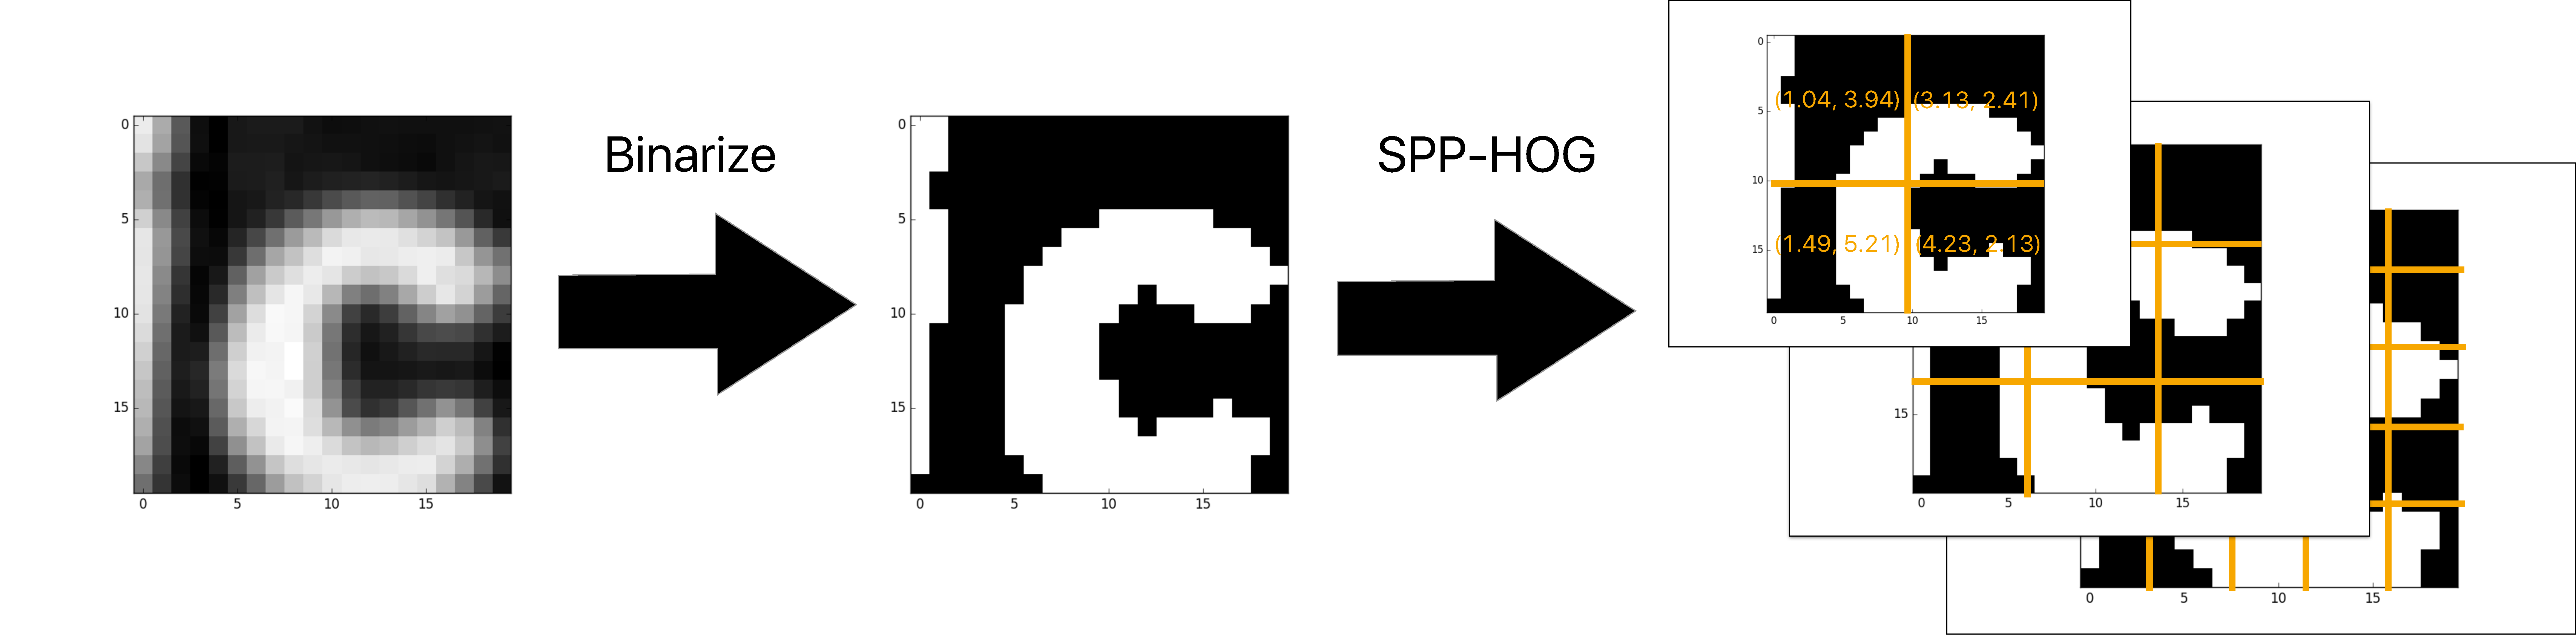
\includegraphics[width=0.8\linewidth]{img/preprocessing.pdf}
    \caption{Preprocessing steps} \label{fig:preprocessing}
\end{figure}

\section{Classifiers}
\subsection{SVC}
Our approach to classifiers was driven by our lack of experience with
using machine learning frameworks.  When starting out we used a
tutorial for recognizing hand written digits provided by scikit which
happened to use a support vector classifier. %link til tutorial?
http://scikit-learn.org/stable/auto_examples/classification/plot_digits_classification.html#example-classification-plot-digits-classification-py
In our first attempt we simply extended the example from sklearn to
create a dataset from 74k-lite to see what kind of performance we
would get.  After getting very lackluster results we first thought
there was an error in our program, a test run using only the a's and
b's predicted only a's which made us spend time debugging.  A quick
look on the datasets revealed why we were wrong: the example we
followed used a set of 10*10 images which were all cleanly written.
Compared to our pictures which featured many different fonts and four
times as many pixels the task of classifying the example images was
much smaller.  Realizing this we tried implementing some preprocessors
to see how our classifiers fared with inputs featuring lower
dimensionality.  Returning to the classifier we resumed our trials
with our arbitrarily chosen SVC.  The standard sklearn SVC
implementation uses an rbf kernel, standing for radial basis function
network.  Because we did not know how rbf worked we decided to try out
a linear kernel instead.  This made sense not only because of the
approachability compared to the complex rbf implementation, but also
because we had a somewhat intuitive understanding of why it could
perform well.  With our radial orientation scheme we predicted that
the amount of angled surfaces in letters would be linearly separable
allowing the linear SVC to perform well.  We can't be sure whether
this intuition was correct, but we got very nice results, handily
beating our initial rbf kernel implementation.  One flaw with using an
svm is that our dataset consists of both small and big letters,
essentially creating "islands" which would make it hard to partition
the feature space into partitions consisting both of the big and small
version of a letter.  We are unsure how the SVM in scikit is
implemented.  It is possible that several clusters may be formed for
the same class which would explain why it performed so well, or
perhaps the SVC found a way to create partitions containing both the
small and the big version for each letter.  The best result we
obtained with a linear classifier was a precision of 0.78 which was
achieved when first binarizing the images and then applying HOG % with
[5, 4, 2] We expected HOG to perform fairly well on images without
applying binarization as HOG should be able to deal with noise.  With
no binarization the classifier reached a score of 0.76 which tells us
that while HOG pulls most of the weight the additional step of
binarization is still worthwhile, yielding an ~8\% reductiong of
missclassifications.  The following table shows the performance of our
SVC using different parameters:

\begin{tabular}{l | l | l}
    Kernel & preprocessing & precision\\ \hline
    Linear & binarization \& HOG & 0.78 \\ \hline
    Linear & binarization & 0.11 \\ \hline
    Linear & HOG & 0.76\\ \hline
\end{tabular}

\subsection{K Nearest neighbors}
In order to test out our theory that an SVC would suffer from
different versions of letters we settled on k nearest neighbors as a
second classifier.  We hypothesized that this method would perform
better based on our suspected weakness of the SVC since nearest
neighbours does not rely on partitioning the feature space.  Our best
performing configuration managed a precision of 0.81 using 10
neighbours linearly weighted by manhattan distance, yielding a fairly
decent improvement.  Not only did K nearest outperform SVC, it also
did so without having to use the binarization preprocessing step.
We're not sure why binarization is nescessary using SVC compared to K
nearest % postuler no greier her..? % The following table shows the
performance of our K nearest classifier using different parameters:
\begin{tabular}{l | l | l | l | l}
    K (neighbors) & weight & distance measure & preprossesing & precision\\ \hline
    10 & linear distance & euclidean & HOG & 0.80\\ \hline
    10 & uniform & HOG & euclidean & 0.79\\ \hline
    5 & uniform & HOG & euclidean & 0.79\\ \hline
    10 & linear & HOG & manhattan & 0.81\\ \hline
    10 & linear & HOG \& binarization & manhattan & 0.81\\ \hline
\end{tabular}
    
\bibliographystyle{plain}
\bibliography{references.bib} 

\end{document}
